%package list
\documentclass{article}
\usepackage[top=3cm, bottom=3cm, outer=3cm, inner=3cm]{geometry}
\usepackage{multicol}
\usepackage{graphicx}
\usepackage{url}
%\usepackage{cite}
\usepackage{hyperref}
\usepackage{array}
%\usepackage{multicol}
\newcolumntype{x}[1]{>{\centering\arraybackslash\hspace{0pt}}p{#1}}
\usepackage{natbib}
\usepackage{pdfpages}
\usepackage{multirow}    
\usepackage[normalem]{ulem}
\useunder{\uline}{\ul}{}
\usepackage{svg}
\usepackage{xcolor}
\usepackage{listings}
\lstdefinestyle{ascii-tree}{
    literate={├}{|}1 {─}{--}1 {└}{+}1 
  }

\lstset{basicstyle=\ttfamily,
  showstringspaces=false,
  commentstyle=\color{red},
  keywordstyle=\color{blue}
}
%\usepackage{booktabs}
\usepackage{caption}
\usepackage{subcaption}
\usepackage{float}
\usepackage{array}

\usepackage{enumitem}


\newcolumntype{M}[1]{>{\centering\arraybackslash}m{#1}}
\newcolumntype{N}{@{}m{0pt}@{}}


%%%%%%%%%%%%%%%%%%%%%%%%%%%%%%%%%%%%%%%%%%%%%%%%%%%%%%%%%%%%%%%%%%%%%%%%%%%%
%%%%%%%%%%%%%%%%%%%%%%%%%%%%%%%%%%%%%%%%%%%%%%%%%%%%%%%%%%%%%%%%%%%%%%%%%%%%
\newcommand{\itemEmail}{vmaldonadov@unsa.edu.pe}
\newcommand{\itemStudent}{Victor Gonzalo Maldonado Vilca}
\newcommand{\itemCourse}{Programación Web 2}
\newcommand{\itemCourseCode}{1702122}
\newcommand{\itemSemester}{III}
\newcommand{\itemUniversity}{Universidad Nacional de San Agustín de Arequipa}
\newcommand{\itemFaculty}{Facultad de Ingeniería de Producción y Servicios}
\newcommand{\itemDepartment}{Departamento Académico de Ingeniería de Sistemas e Informática}
\newcommand{\itemSchool}{Escuela Profesional de Ingeniería de Sistemas}
\newcommand{\itemAcademic}{2024 - A}
\newcommand{\itemInput}{Del 16 de mayo de 2024}
\newcommand{\itemOutput}{Al 15 de junio de 2024}
\newcommand{\itemPracticeNumber}{07}
\newcommand{\itemTheme}{Django Templates}
%%%%%%%%%%%%%%%%%%%%%%%%%%%%%%%%%%%%%%%%%%%%%%%%%%%%%%%%%%%%%%%%%%%%%%%%%%%%
%%%%%%%%%%%%%%%%%%%%%%%%%%%%%%%%%%%%%%%%%%%%%%%%%%%%%%%%%%%%%%%%%%%%%%%%%%%%

\usepackage[english,spanish]{babel}
\usepackage[utf8]{inputenc}
\AtBeginDocument{\selectlanguage{spanish}}
\renewcommand{\figurename}{Figura}
\renewcommand{\refname}{Referencias}
\renewcommand{\tablename}{Tabla} %esto no funciona cuando se usa babel
\AtBeginDocument{%
	\renewcommand\tablename{Tabla}
}

\usepackage{fancyhdr}
\pagestyle{fancy}
\fancyhf{}
\setlength{\headheight}{30pt}
\renewcommand{\headrulewidth}{1pt}
\renewcommand{\footrulewidth}{1pt}
\fancyhead[L]{\raisebox{-0.2\height}{
\includegraphics[width=3cm]{img/logo_episunsa.png}}}
\fancyhead[C]{\fontsize{7}{7}\selectfont	\itemUniversity \\ \itemFaculty \\ \itemDepartment \\ \itemSchool \\ \textbf{\itemCourse}}
\fancyhead[R]{\raisebox{-0.2\height}{
\includegraphics[width=1.2cm]{img/logo_abet}}}
\fancyfoot[L]{Victor M.}
\fancyfoot[C]{\itemCourse}
\fancyfoot[R]{Página \thepage}

% para el codigo fuente
\usepackage{listings}
\usepackage{color, colortbl}
\definecolor{dkgreen}{rgb}{0,0.6,0}
\definecolor{gray}{rgb}{0.5,0.5,0.5}
\definecolor{mauve}{rgb}{0.58,0,0.82}
\definecolor{codebackground}{rgb}{0.95, 0.95, 0.92}
\definecolor{tablebackground}{rgb}{0.8, 0, 0}
\definecolor{gitgreen}{RGB}{40, 160, 40}
\definecolor{gitred}{RGB}{255, 0, 0}
\definecolor{gitgray}{RGB}{128, 128, 128}

\lstset{frame=tb,
	language=bash,
	aboveskip=3mm,
	belowskip=3mm,
	showstringspaces=false,
	columns=flexible,
	basicstyle={\small\ttfamily},
	numbers=none,
	numberstyle=\tiny\color{gray},
	keywordstyle=\color{blue},
	commentstyle=\color{dkgreen},
	stringstyle=\color{mauve},
	breaklines=true,
	breakatwhitespace=true,
	tabsize=3,
	backgroundcolor= \color{codebackground},
}

\begin{document}
	
	\vspace*{10px}
	
	\begin{center}	
		\fontsize{17}{17} \textbf{ Informe de Django 3 Templates}
	\end{center}
	\centerline{\textbf{\Large Tema: \itemTheme}}
	%\vspace*{0.5cm}	

	\begin{flushright}
		\begin{tabular}{|M{2.5cm}|N|}
			\hline 
			\rowcolor{tablebackground}
			\color{white} \textbf{Nota}  \\
			\hline 
			     \\[30pt]
			\hline 			
		\end{tabular}
	\end{flushright}	

	\begin{table}[H]
		\begin{tabular}{|x{4.7cm}|x{4.8cm}|x{4.8cm}|}
			\hline 
			\rowcolor{tablebackground}
			\color{white} \textbf{Estudiante} & \color{white}\textbf{Escuela}  & \color{white}\textbf{Asignatura}   \\
			\hline 
			{\itemStudent \par \itemEmail} & \itemSchool & {\itemCourse \par Semestre: \itemSemester \par Código: \itemCourseCode}     \\
			\hline 			
		\end{tabular}
	\end{table}		
	
	\begin{table}[H]
		\begin{tabular}{|x{4.7cm}|x{4.8cm}|x{4.8cm}|}
			\hline 
			\rowcolor{tablebackground}
			\color{white}\textbf{Tarea} & \color{white}\textbf{Tema}  & \color{white}\textbf{Duración}   \\
			\hline 
			\itemPracticeNumber & \itemTheme & 2 horas   \\
			\hline 
		\end{tabular}
	\end{table}
	
	\begin{table}[H]
		\begin{tabular}{|x{4.7cm}|x{4.8cm}|x{4.8cm}|}
			\hline 
			\rowcolor{tablebackground}
			\color{white}\textbf{Semestre académico} & \color{white}\textbf{Fecha de inicio}  & \color{white}\textbf{Fecha de entrega}   \\
			\hline 
			\itemAcademic & \itemInput &  \itemOutput  \\
			\hline 
		\end{tabular}
	\end{table}
%%%%%%%%%%%%%%%%%%%%

  \section{Introducción}
    Las plantillas en Django son archivos HTML que permiten generar contenido dinámico al integrar código Python. 
    Se almacenan en el directorio templates, se extienden usando herencia, y se manipulan con etiquetas y variables 
    de Django para mostrar datos dinámicos y aplicar filtros. Son fundamentales para crear interfaces web dinámicas 
    y flexibles en aplicaciones Django.
  
%%%%%%%%%%%%%%%%%%%%

  \section{Objetivos}
    \begin{itemize}
      \item Generar contenido HTML dinámico basado en datos de la aplicación.
      \item Reutilizar código mediante la creación de plantillas base y herencia.
      \item Mantener la separación entre la lógica y la presentación en las aplicaciones web.
      \item Crear interfaces interactivas utilizando etiquetas, variables y filtros.
      \item Optimizar el desarrollo al agilizar el manejo de la presentación de datos en Django.
    \end{itemize}

%%%%%%%%%%%%%%%%%%%%
 
	\section{Tarea}
    \begin{itemize}
      \item En esta tarea deberá seguir las diapositivas de DJango03, dentro de un proyecto git local.
      \item Deberá hacer un commit por cada paso y deberá usar branch para hacer sus experimentos o pruebas.
      \item La entrega de la tarea consistirá de texto con las respuestas a las preguntas de las diapositivas (incluya el enunciado de la diapositiva) y una captura de pantalla (deberá incrustar la captura de pantalla al inicio de su texto de respuesta) del siguiente comando:   
        \begin{verbatim}
          git log --graph --pretty=oneline --abbrev-commit --all
        \end{verbatim}
      \item NO INCLUYA commits de tareas pasadas.
      \item Cada commit debe ser realizado con un mensaje descriptivo del paso de la diapositiva que estuvo siguiendo
    \end{itemize}
  
%%%%%%%%%%%%%%%%%%%% 
 
  \section{Entregables}
    \begin{itemize}
      \item Informe hecho en Latex.
      \item \textbf{texto: }Respuestas a las preguntas de las diapositivas 
      \item Captura de pantalla del siguiente comando:
        \begin{verbatim}
          git log --graph --pretty=oneline --abbrev-commit --all
        \end{verbatim}
      \item \textbf{Extra: }URL - Repositorio GitHub
    \end{itemize}
  
%%%%%%%%%%%%%%%%%%%%    
		
	\section{Equipos, materiales y temas utilizados}
    \begin{itemize}
      \item \textbf{Sintaxis de plantillas en Django}.
      \item \textbf{Herencia de plantillas y bloques}.
      \item \textbf{Contexto de plantillas y vistas en Django}.
      \item \textbf{Uso avanzado de plantillas}.
    \end{itemize}

%%%%%%%%%%%%%%%%%%%%

	\section{Respuestas a las Preguntas dejadas en las Diapositivas}
    \begin{enumerate}
      \item \textbf{Pruebe qué ocurre si no incluímos el campo “donador” en el formulario¿De qué se trata este error?}
        \newline
        \textbf{Respuesta: }Este error trata de que si el campo 'donador' es requerido en el modelo Persona y no se 
        incluye en el formulario al intentar guardar un objeto de Persona con este formulario, se producirá un error 
        de validación. Debido a que Django espera que todos los campos requeridos sean proporcionados al crear o actualizar 
        una instancia del modelo.
      \item \textbf{¿Cómo se puede solucionar?}
        \newline
        \textbf{Respuesta: }La solución más obvia es volver a agregar el campo en el formulario. 
        Otra solución es establecer un valor por defecto usando 'default=True' o 'default=False'. Recordemos que el valor 
        por defecto cambiará dependiendo del tipo de dato que sea el campo, en este caso, es booleano.
      \item \textbf{Del ejemplo anterior vemos que la vista se llama primero con GET y luego con POST ¿En qué momento se hace llamada GET y en qué momento se hace la llamada POST?}
        \newline
        \textbf{Respuesta: }La llamada GET se realiza al enviar el formulario con 'method=GET', mientras que la llamada POST se 
        realiza al enviar el formulario con 'method=POST' y el token CSRF. Pero su principal diferencia es que el método GET 
        se usa comúnmente para solicitar recursos o enviar datos de manera visible en la URL, mientras que el método POST se 
        usa para enviar datos de manera más segura y sin mostrarlos directamente en la URL.  
    \end{enumerate}

%%%%%%%%%%%%%%%%%%%%

	\section{Captura de Pantalla}
    \begin{figure}[H]
      \centering
      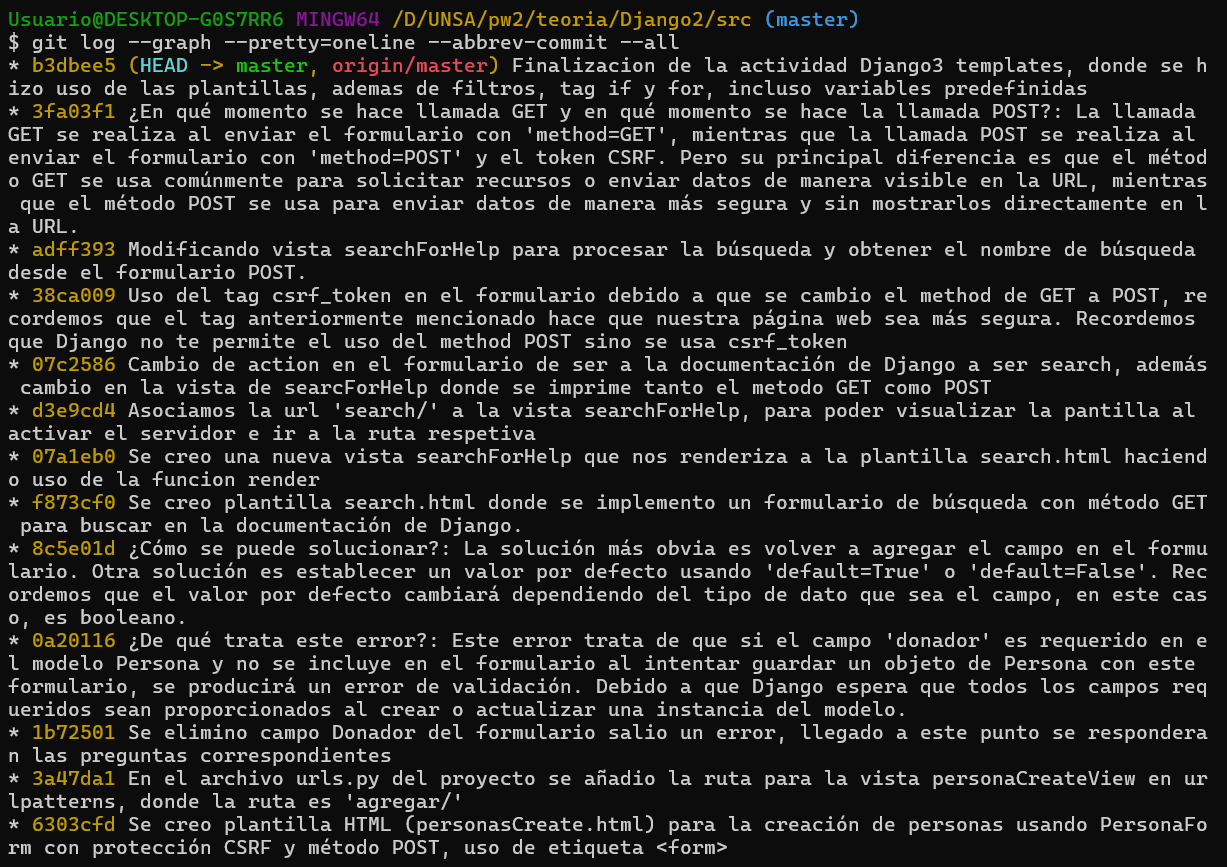
\includegraphics[width=1\textwidth, keepaspectratio]{img/commits1.png}
      \caption{Primera Parte commits}
    \end{figure}
    \newpage
    \begin{figure}[H]
      \centering
      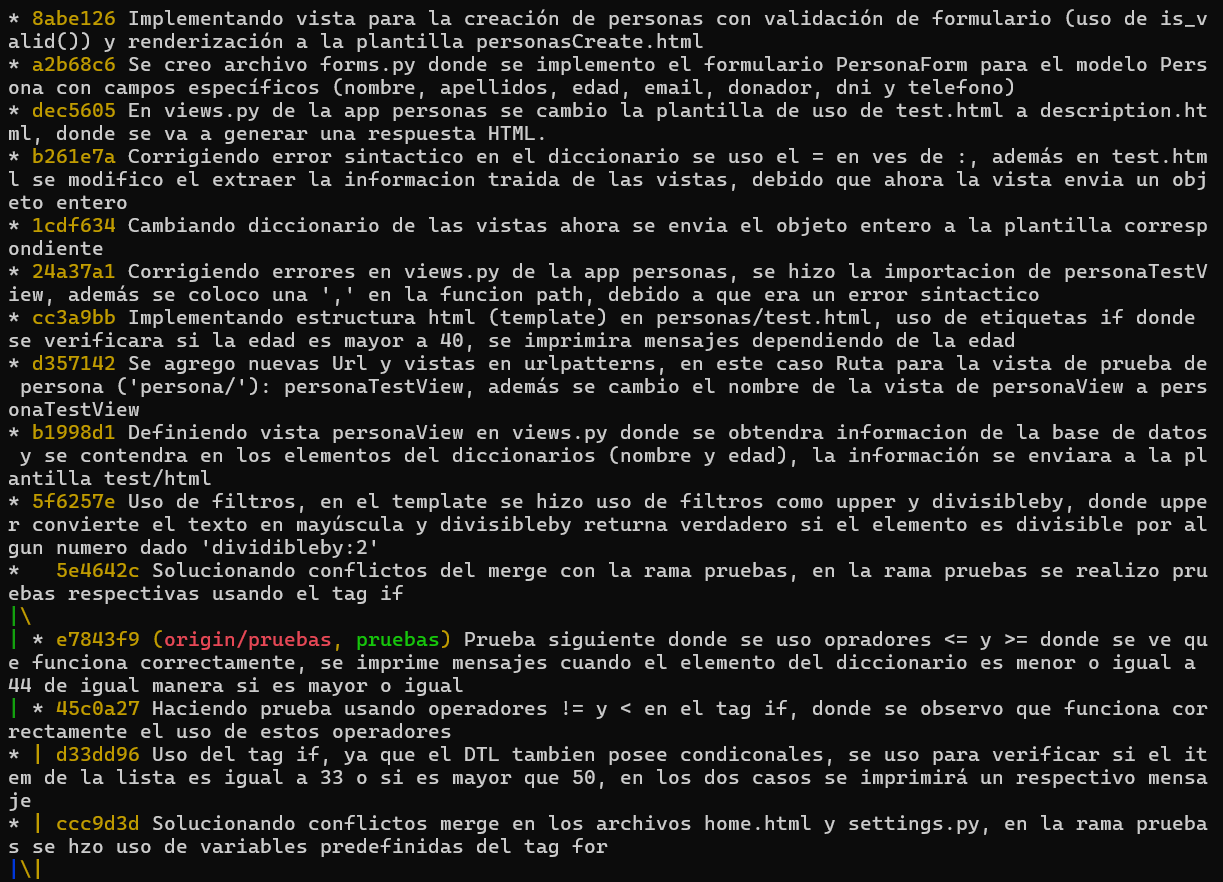
\includegraphics[width=1\textwidth, keepaspectratio]{img/commits2.png}
      \caption{Segunda Parte commits}
    \end{figure}
    \begin{figure}[H]
      \centering
      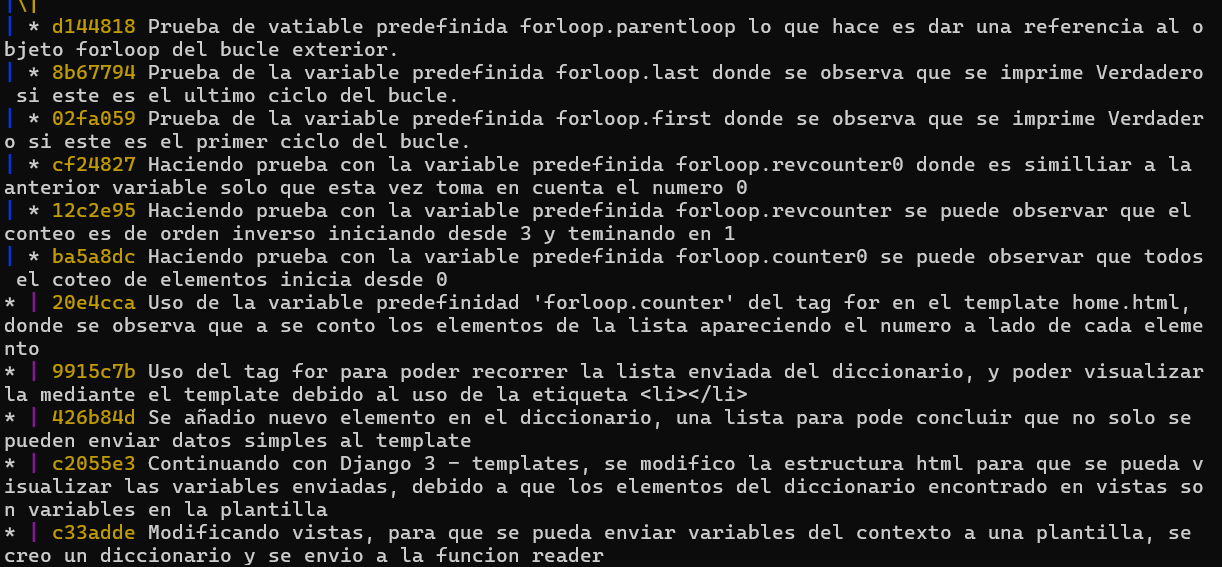
\includegraphics[width=1\textwidth, keepaspectratio]{img/commits3.png}
      \caption{Tercera Parte commits}
    \end{figure}

%%%%%%%%%%%%%%%%%%%%

  \section{URL de Repositorio Github}
    \begin{itemize}
      \item URL del Repositorio GitHub.
      \item \url{https://github.com/Victor-Gonzalo-Maldonado-Vilca/Django2.git}
    \end{itemize}

%%%%%%%%%%%%%%%%%%%%

  \section{Metodología}
    \textit{Debido a que es un proyecto continuo - La metodología ya esta empleada en las actividades de Django1 y Django2}
    
%%%%%%%%%%%%%%%%%%%%

  \section{Desarrollo del trabajo}
    \textit{Continuamos a partir del proyecto realizado en Django 2}

%%%%%%%%%%%%

  \subsection{Modelos -- Aplicación personas}
    El modelo \texttt{Persona} en Django define los atributos que se utilizarán para almacenar información sobre una persona en la base de datos. Cada atributo tiene un tipo de datos específico y ciertas reglas asociadas:
    \begin{itemize}
        \item \texttt{nombre}: Se trata de un campo de texto que puede almacenar hasta 100 caracteres y es obligatorio.
        \item \texttt{apellidos}: Otro campo de texto que también puede contener hasta 100 caracteres y debe ser completado.
        \item \texttt{edad}: Este campo guarda un número entero que representa la edad de la persona.
        \item \texttt{email}: Aquí se almacena la dirección de correo electrónico de la persona, con un límite de 100 caracteres.
        \item \texttt{donador}: Un campo booleano que indica si la persona es donante o no. Por defecto, se establece como \texttt{False} si no se especifica lo contrario.
        \item \texttt{dni}: Se utiliza para guardar el número de documento nacional de identidad (DNI) de la persona, aunque este campo puede quedar vacío si no se proporciona.
        \item \texttt{telefono}: Este campo guarda el número de teléfono de la persona y también puede quedar sin completar si no se desea proporcionar esta información.
    \end{itemize}
    Estos atributos permiten almacenar información relevante sobre una persona de manera organizada en la base de datos de la aplicación Django. Después se harán las migraciones 
    correspondientes.
    \begin{lstlisting}[language=Python, caption={Modelo Persona}]
      class Persona(models.Model):
        nombre    = models.CharField(max_length = 100, blank=False)
        apellidos = models.CharField(max_length = 100, blank=False)
        edad      = models.IntegerField()
        email     = models.CharField(max_length = 100)
        donador   = models.BooleanField(default=False)
        dni       = models.CharField(max_length = 8, null=True)
        telefono  = models.CharField(max_length = 9, null=True)
    \end{lstlisting}
    \newpage
    
%%%%%%
  
  \subsubsection{Examinando los objetos del Modelo}
    \begin{figure}[H]
      \centering
      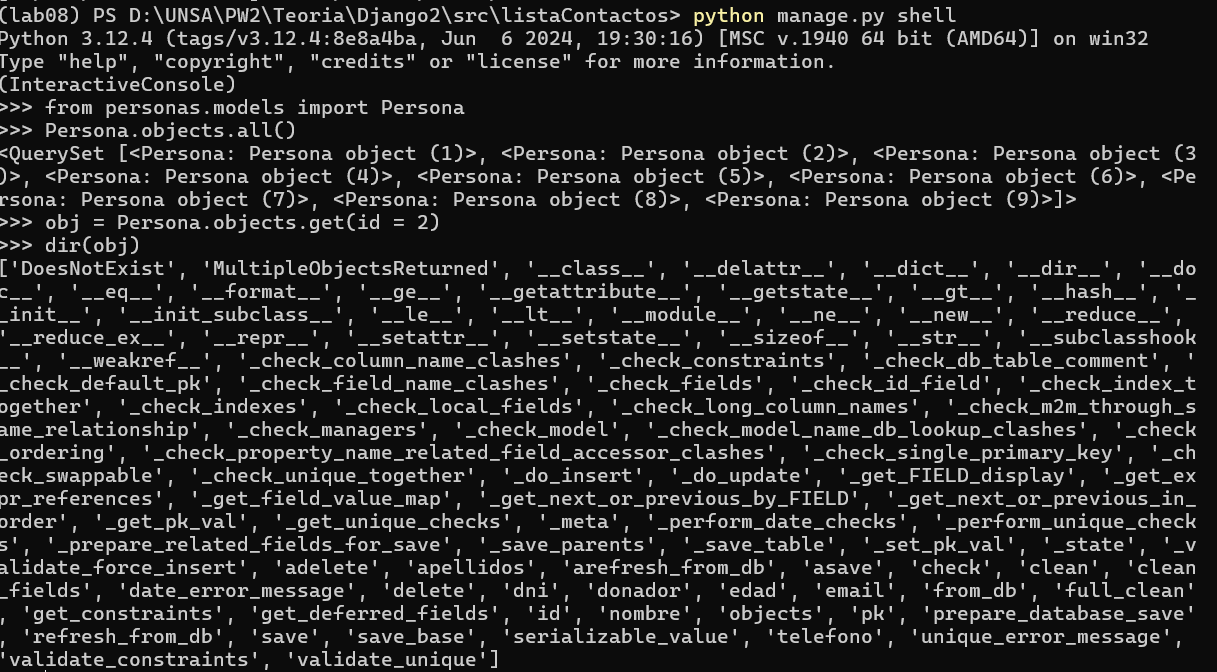
\includegraphics[width=1\textwidth, keepaspectratio]{img/examinar.png}
      \caption{Examinar objetos del Modelo}
    \end{figure}
    
%%%%%%%%%%%%

  \subsection{Vistas -- Aplicación personas}
    Estos son tres views en Django. personaTestView muestra los detalles de una persona según su ID. personaCreateView procesa 
    un formulario para crear una nueva persona. searchForHelp busca ayuda mediante un formulario de búsqueda y muestra los resultados.
    \begin{lstlisting}[language=python]
      from django.shortcuts import render
      from .models import Persona
      from .forms import PersonaForm

      # Create your views here.

      def personaTestView(request):
          obj = Persona.objects.get(id = 1)
          context = {
              'objeto': obj,
          }
          return render(request, 'personas/description.html', context)

      def personaCreateView(request):
          form = PersonaForm(request.POST or None)
          if form.is_valid():
              form.save()
              form = PersonaForm()
              
          context = {
              'form': form
          }
          
          return render(request, 'personas/personasCreate.html', context)
          
      def searchForHelp(request):
          print(request)
          if request.method == 'POST':
              nombre = request.POST.get('q')
              print(nombre)
          context = {}
          return render(request, 'personas/search.html', context)
    \end{lstlisting}

  
%%%%%%%%%%%%

  \subsection{Vistas -- Aplicación inicio}
    Estos son dos views básicos en Django. myHomeView renderiza una plantilla llamada "home.html" con un contexto que 
    incluye un texto, un número y una lista. Mientras tanto, anotherView devuelve directamente una respuesta HTTP con 
    un título en formato HTML.
    \begin{lstlisting}[language=python]
      from django.shortcuts import render
      from django.http import HttpResponse

      # Create your views here.

      def myHomeView(request, *args, **kwargs):
          myContext = {
              'myText': 'Esto es sobre nosostros',
              'myNumber': 123,
              'myList': [33, 44, 55],
          }
          return render(request, "home.html", myContext)
          
      def anotherView(request):
          return HttpResponse('<h1>Solo otra pagina</h1>')
    \end{lstlisting}

  
%%%%%%%%%%%%

  \subsection{URLs -- proyecto listaContactos}
    Esto configura las rutas URL para las diferentes vistas de tu aplicación Django:
    \begin{itemize}
      \item La primera ruta, \texttt{'admin/'}, permite acceder al panel de administración de Django a través de la URL \texttt{/admin/}.  
      \item La segunda ruta, \texttt{''} (página de inicio), está asociada a la vista \texttt{myHomeView} definida en \texttt{inicio.views}. Esta ruta representa la página principal de tu aplicación y se accede a través de la URL base del sitio.   
      \item La tercera ruta, \texttt{'another/'}, está asociada a la vista \texttt{anotherView} de \texttt{inicio.views}. Esta ruta permite acceder a una página adicional dentro de tu aplicación mediante la URL \texttt{/another/}.   
      \item La cuarta ruta, \texttt{'persona/'}, está asociada a la vista \texttt{personaTestView} de \texttt{personas.views}. Al acceder a esta URL (\texttt{/persona/}), se mostrará la información de una persona específica.  
      \item La quinta ruta, \texttt{'agregar/'}, está asociada a la vista \texttt{personaCreateView} de \texttt{personas.views}. Esta ruta permite agregar una nueva persona a través de la URL \texttt{/agregar/}.    
      \item La sexta ruta, \texttt{'search/'}, está asociada a la vista \texttt{searchForHelp} de \texttt{personas.views}. Esta ruta se utiliza para buscar ayuda dentro de la aplicación y se accede mediante la URL \texttt{/search/}.
    \end{itemize}

    \begin{lstlisting}[language=python]
      from django.contrib import admin
      from django.urls import path
      from inicio.views import myHomeView, anotherView
      from personas.views import personaTestView, personaCreateView, searchForHelp

      urlpatterns = [
          path('admin/', admin.site.urls),
          path('', myHomeView, name='Pagina de Inicio'),
          path('another/', anotherView, name='otro'),
          path('persona/', personaTestView, name='testViewPersona'),
          path('agregar/', personaCreateView, name='createPersona'),
          path('search/', searchForHelp, name='buscar'),
      ]
    \end{lstlisting}

  
%%%%%%%%%%%%%%%%%%%%%

  \section{Templates}
  
%%%%%%%%%%%%

  \subsection{Plantilla home.html}
    El siguiente código define una página HTML que utiliza plantillas de Django. La página se extiende de otra plantilla 
    llamada \texttt{base.html}, lo que significa que hereda su estructura y estilos, y luego agrega contenido adicional en 
    un bloque específico llamado \texttt{content}.
    Dentro del bloque \texttt{content}, se incluyen varios elementos HTML:
      \begin{itemize}
        \item Un encabezado de nivel 2 (\texttt{<h2>}) que muestra el texto "Hola Mundo desde Django".
        \item Un encabezado de nivel 3 (\texttt{<h3>}) con el texto "Con Templates".
        \item Un párrafo (\texttt{<p>}) que muestra el contenido de la variable \texttt{myText} en mayúsculas y truncado a 16 caracteres, seguido por el valor de la variable \texttt{myNumber}.
        \item Una lista desordenada (\texttt{<ul>}) generada mediante un bucle \texttt{for}, donde cada elemento de la lista se obtiene de la variable \texttt{myList}.
        \item Cada elemento de la lista muestra su posición utilizando \texttt{forloop.counter} y el valor de la variable incrementado en 2 usando \texttt{|add:2}.
        \item Se incluyen condiciones \texttt{if}, \texttt{elif} y \texttt{else} dentro del bucle para agregar texto adicional según el valor de cada elemento en \texttt{myList}.
      \end{itemize}
    \begin{lstlisting}[language=html]
      <!DOCTYPE HTML>
      <html>
        <head>
          <title>Template Base</title>
        </head>
        <body>
          
          
          <h2>Hola Mundo desde Django</h2>
          <h3>Con Templates</h3>
          <p>
            {{ myText|upper|truncatechars:"16" }},
            {{ myNumber }}
          </p>
          <ul>
            
              <li>{{forloop.counter}} - {{ myItem|add:2 }}
              
                - Este numero es magico
              
                - Este numero es par
              
                - Este numero es mayor que 50
              
              </li>
            
          </ul>
          
        </body>
      </html>
    \end{lstlisting}
    \textbf{EJECUCIÓN: }
    \begin{figure}[H]
      \centering
      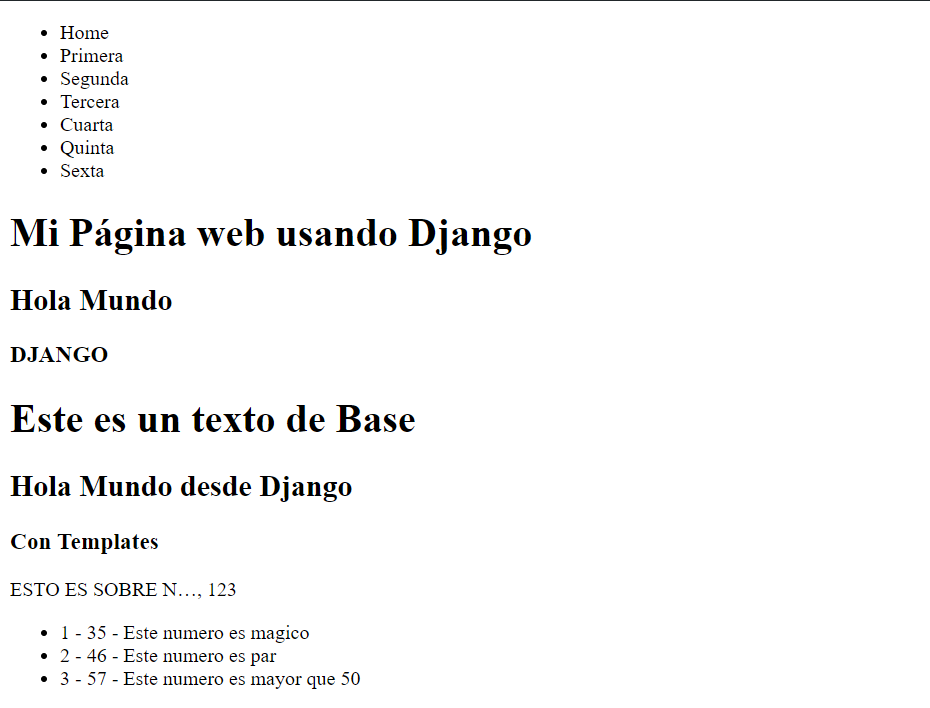
\includegraphics[width=1\textwidth, keepaspectratio]{img/ejecucion1.png}
      \caption{Ejecución}
    \end{figure}
    \newpage
    
%%%%%%%%%%%%

  \subsection{Plantilla description.html -- templates/personas/}
    Este código HTML es una plantilla de Django que extiende otra plantilla llamada 'base.html' y define un bloque de 
    contenido. Dentro de este bloque, se muestra el nombre y la edad de un objeto utilizando variables de Django ({{ objeto.nombre }} 
    y {{ objeto.edad }}). Además, incluye una condición para mostrar un mensaje basado en la edad del objeto: si la edad es mayor 
    que 40, muestra "debe cuidarse del colesterol", de lo contrario, muestra "puede comer lo que quiera".

    \begin{lstlisting}[language=html]
      <!DOCTYPE HTML>
      <html>
        <head>
          <meta charset="UTF-8"/>
          <meta name="viewport" content="width=device-width, initial-scale=1.0"/>
          <title>test</title>
        </head>
        <body>
          
          
          <h1>{{objeto.nombre}}</h1>
          <h2>
            
            debe cuidarse del colesterol
            
            puede comer lo que quiera
            
          </h2>
          
        </body>
      </html>
    \end{lstlisting}
    \newpage
    \textbf{EJECUCIÓN: }
    \begin{figure}[H]
      \centering
      
\includegraphics[width=1\textwidth, keepaspectratio]{img/ejecucion2.png}
      \caption{Ejecución}
    \end{figure}
  
%%%%%%%%%%%%

  \subsection{Plantilla personasCreate.html -- templates/personas/}
    Este código HTML es una plantilla de Django que se utiliza para crear un nuevo objeto de tipo Persona. La plantilla extiende 
    otra plantilla llamada 'base.html' y define un bloque de contenido donde se encuentra un formulario. Este formulario utiliza 
    el método POST y está protegido contra ataques CSRF mediante el token 'csr ftoken'. El formulario se renderiza utilizando 
    el objeto 'form.as p', que genera los campos del formulario como párrafos. Finalmente, hay un botón de tipo submit con el texto 
    'Grabar' para enviar el formulario y crear el objeto Persona.

    \begin{lstlisting}[language=html]
      <!DOCTYPE HTML>
      <html>
        <head>
          <meta charset="UTF-8"/>
          <meta name="viewport" content="width=device-width, initial-scale=1.0"/>
          <title>Create Persona</title>
        </head>
        <body>
          
          
          <form method='POST'> 
            {{ form.as_p }}
            <input type='submit' value='Grabar'/>
          </form>
          
        </body>
      </html>
    \end{lstlisting}
    \textbf{EJECUCIÓN: }
    \begin{figure}[H]
      \centering
      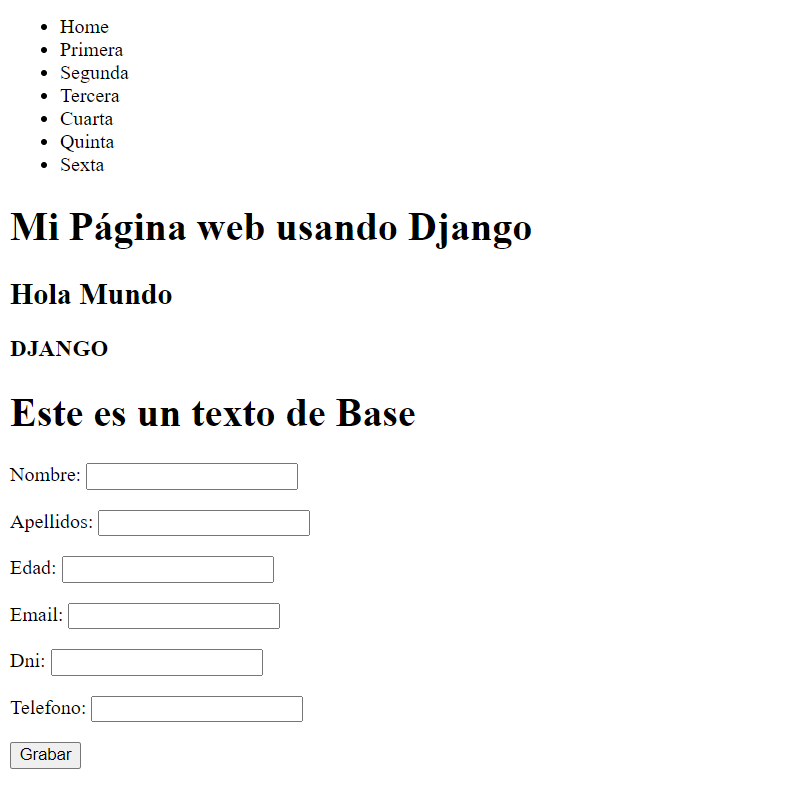
\includegraphics[width=1\textwidth, keepaspectratio]{img/ejecucion3.png}
      \caption{Ejecución}
    \end{figure}

%%%%%%%%%%%%

  \subsection{Plantilla search.html -- templates/personas/}
    Esta plantilla HTML forma parte de un formulario de búsqueda en Django. Está diseñada para integrarse con otra 
    plantilla llamada 'base.html' y presenta un bloque de contenido que incluye el formulario. Utiliza el método 
    POST para enviar datos y asegura la protección contra ataques CSRF con un token especial. Dentro del formulario, 
    se encuentra un campo de texto para ingresar el término de búsqueda y un botón para activar la búsqueda.

    \begin{lstlisting}[language=html]
      <!DOCTYPE HTML>
      <html>
        <head>
          <meta charset="UTF-8"/>
          <meta name="viewport" content="width=device-width, initial-scale=1.0"/>
          <title>Create Persona</title>
        </head>
        <body>
          
          
          <form method='POST'> 
            {{ form.as_p }}
            <input type='submit' value='Grabar'/>
          </form>
          
        </body>
      </html>
    \end{lstlisting}
    \textbf{EJECUCIÓN: }
    \begin{figure}[H]
      \centering
      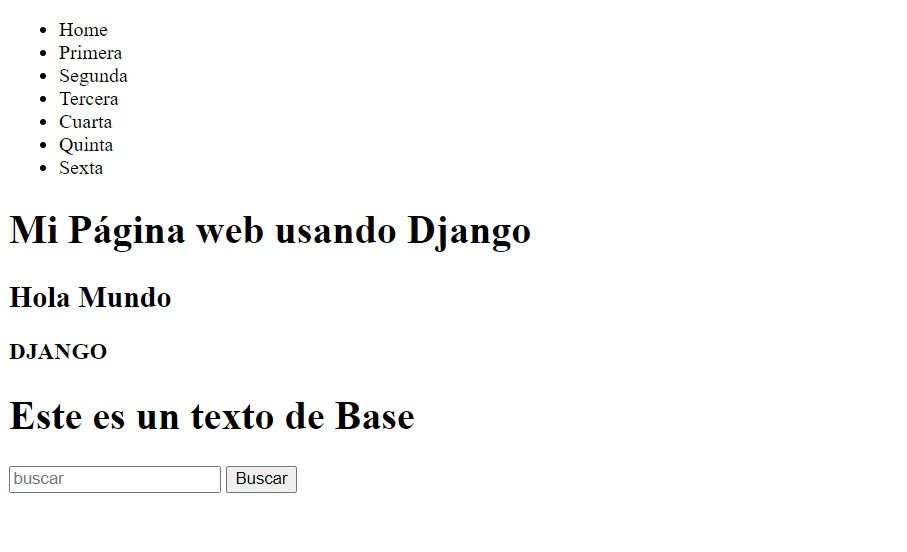
\includegraphics[width=1\textwidth, keepaspectratio]{img/ejecucion4.png}
      \caption{Ejecución}
    \end{figure}
    \begin{figure}[H]
      \centering
      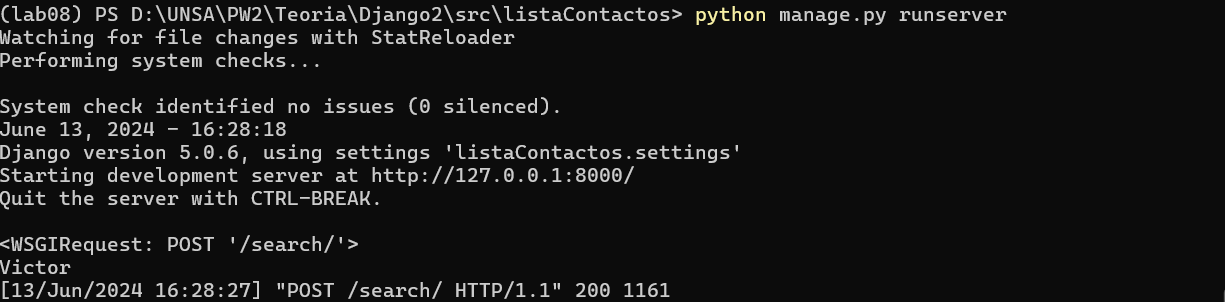
\includegraphics[width=1\textwidth, keepaspectratio]{img/post.png}
      \caption{servidor}
    \end{figure}
    \begin{figure}[H]
      \centering
      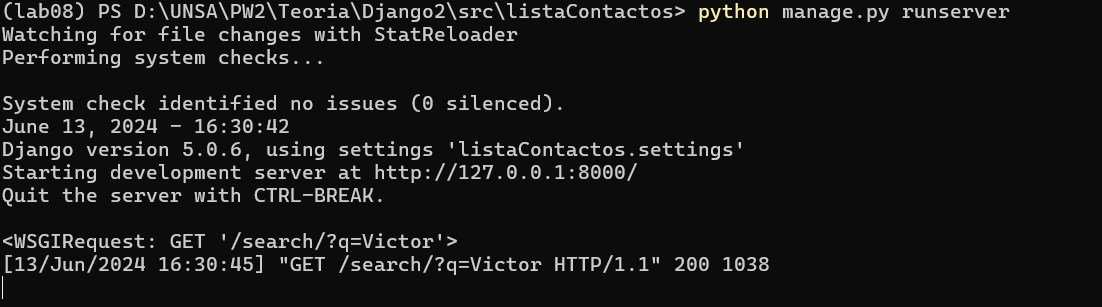
\includegraphics[width=1\textwidth, keepaspectratio]{img/get.png}
      \caption{servidor}
    \end{figure}
  
%%%%%%%%%%%%

  \subsection{Ejecución del servidor}
  Este siguiente comando inicia el servidor local de Django. Una vez ejecutado, el servidor estará disponible por defecto en la dirección 
  \texttt{http://127.0.0.1:8000/}. Desde esta dirección, se puede acceder a las diferentes vistas y funcionalidades del 
  proyecto Django.
  \begin{lstlisting}[language=bash]
    python manage.py runserver
  \end{lstlisting}
  
%%%%%%%%%%%%%%%%%%%%

  \section{Recomensaciones}
  \begin{itemize}
    \item Asegurarse siempre de incluir todos los campos requeridos en los formularios de Django para evitar errores de validación. 
    Utilizar valores por defecto de manera cuidadosa y coherente, especialmente en campos booleanos u otros tipos de datos sensibles.
  \end{itemize}

%%%%%%%%%%%%%%%%%%%%

  \section{Conclusiones}
  \begin{itemize}
    \item El uso efectivo de plantillas en Django permite una optimización significativa del frontend de las aplicaciones web. 
    Al separar la lógica de presentación del código Python, se facilita el mantenimiento y la modificación de la interfaz de 
    usuario, lo que resulta en una experiencia más agradable para los usuarios finales.
    \item Las plantillas en Django proporcionan una gran flexibilidad y capacidad de reutilización de componentes de interfaz. 
    Esto permite construir interfaces dinámicas y personalizadas de manera eficiente, aprovechando la capacidad de Django para 
    gestionar de forma efectiva la lógica de negocio y la presentación de datos en las aplicaciones web.
  \end{itemize}
  
%%%%%%%%%%%%%%%%%%%%
	\newpage
	\subsection{\textcolor{red}{Rúbrica para el contenido del Informe y demostración}}
	\begin{itemize}			
		\item El alumno debe marcar o dejar en blanco en celdas de la columna \textbf{Checklist} si cumplio con el ítem correspondiente.
		\item Si un alumno supera la fecha de entrega,  su calificación será sobre la nota mínima aprobada, siempre y cuando cumpla con todos lo items.
		\item El alumno debe autocalificarse en la columna \textbf{Estudiante} de acuerdo a la siguiente tabla:
	
		\begin{table}[ht]
			\caption{Niveles de desempeño}
			\begin{center}
			\begin{tabular}{ccccc}
    			\hline
    			 & \multicolumn{4}{c}{Nivel}\\
    			\cline{1-5}
    			\textbf{Puntos} & Insatisfactorio 25\%& En Proceso 50\% & Satisfactorio 75\% & Sobresaliente 100\%\\
    			\textbf{2.0}&0.5&1.0&1.5&2.0\\
    			\textbf{4.0}&1.0&2.0&3.0&4.0\\
    		\hline
			\end{tabular}
		\end{center}
	\end{table}	
	

	\end{itemize}

 
	
	\begin{table}[H]
		\caption{Rúbrica para contenido del Informe y demostración}
		\setlength{\tabcolsep}{0.5em} % for the horizontal padding
		{\renewcommand{\arraystretch}{1.5}% for the vertical padding
		%\begin{center}
		\begin{tabular}{|p{2.7cm}|p{7cm}|x{1.3cm}|p{1.2cm}|p{1.5cm}|p{1.1cm}|}
			\hline
    		\multicolumn{2}{|c|}{Contenido y demostración} & Puntos & Checklist & Estudiante & Profesor\\
			\hline
			\textbf{1. GitHub} & Hay enlace URL activo del directorio para el  laboratorio hacia su repositorio GitHub con código fuente terminado y fácil de revisar. &2 &X &2 & \\ 
			\hline
			\textbf{2. Commits} &  Hay capturas de pantalla de los commits más importantes con sus explicaciones detalladas. (El profesor puede preguntar para refrendar calificación). &4 &X &4 & \\ 
			\hline 
			\textbf{3. Código fuente} &  Hay porciones de código fuente importantes con numeración y explicaciones detalladas de sus funciones. &2 &X &2 & \\ 
			\hline 
			\textbf{4. Ejecución} & Se incluyen ejecuciones/pruebas del código fuente  explicadas gradualmente. &2 &X &2 & \\ 
			\hline			
			\textbf{5. Pregunta} & Se responde con completitud a la pregunta formulada en la tarea.  (El profesor puede preguntar para refrendar calificación).  &2 &X &2 & \\ 
			\hline	
			\textbf{6. Fechas} & Las fechas de modificación del código fuente estan dentro de los plazos de fecha de entrega establecidos. &2 &X &2 & \\ 
			\hline 
			\textbf{7. Ortografía} & El documento no muestra errores ortográficos. &2 &X &2 & \\ 
			\hline 
			\textbf{8. Madurez} & El Informe muestra de manera general una evolución de la madurez del código fuente,  explicaciones puntuales pero precisas y un acabado impecable.   (El profesor puede preguntar para refrendar calificación).  &4 &X &4 & \\ 
			\hline
			\multicolumn{2}{|c|}{\textbf{Total}} &20 & &20 & \\ 
			\hline
		\end{tabular}
		%\end{center}
		%\label{tab:multicol}
		}
	\end{table}


%%%%%%%%%%%%%%%%%%%%%%%%%%%%%%%%%%%%%%%%%%%%%%%%%%%%%%%%%%%%%%%%%%%
	
  \newpage
  \section{Referencias}
  \begin{itemize}
    \item \url{https://docs.djangoproject.com/en/5.0/}
    \item \url{https://docs.github.com/es}
    \item \url{https://git-scm.com/doc}
  \end{itemize}
  
%%%%%%%%%%%%%%%%%%%% 
%\clearpage
%\bibliographystyle{apalike}
%\bibliographystyle{IEEEtranN}
%\bibliography{bibliography}
			
\end{document}
